\section{Conclusiones}

\begin{frame}{Sobre ShaderToy}
\begin{itemize}
    \item Este fue un taller básico, hay muchas cosas por experimentar y aprender.
    \item Yo empece leyendo \href{https://inspirnathan.com/posts/47-shadertoy-tutorial-part-1}{este tutorial} y me sirvió mucho.
    \item Aunque vimos como usar Ray Marching en el contexto de ShaderToy, ambas cosas no están necesariamente unidas.
    \begin{itemize}
        \item Se pueden hacer shaders en Shader Toy usando otras técnicas además de Ray Marching.
        \item Se puede utilizar Ray Marching, sin usar el paradigma de \say{Dibujar el mundo en dos triángulos}
    \end{itemize}
    \item El sitio web de ShaderToy no es el único entorno donde puedes experimentar con shaders de juguete.
\end{itemize}
\end{frame}

\begin{frame}{Shaders de juguete}
\begin{itemize}
     \item Hay como tres \say{familias} de shaders en Shader Toy.
     \begin{enumerate}
        \item Técnicas generativas
        \item Técnicas de 2D
        \item Trazadores de rayos.         
     \end{enumerate}
     \item Cualquiera de las tres familias puede desarrollarse mucho más allá de lo que vimos en este taller.
     \item Eso sin mencionar shaders, que usan alguna combinación de técnicas.
     \item También puedes investigar acerca de herramientas de ShaderToy no vistas aquí.
     \begin{itemize}
        \item Canales
        \item Otras formas de interacción
        \item Buffers  
     \end{itemize}
     \item Por supuesto, leer shaders escritos por otras personas en ShaderToy
 \end{itemize}
\end{frame}


\begin{frame}{Técnicas de 2D dimensiones}
\begin{columns}
\column[t]{0.5\textwidth}
    \begin{itemize}
         \item Puedes leer el \href{https://thebookofshaders.com/05/}{libro de los shaders}: el capítulo de Algorithmic drawing
         \item Leer el libro de \href{https://natureofcode.com/}{Nature of code}, los primeros capítulos
         \item Estas son \emph{técnicas generales de GC}, que puedes adaptar para hacer shaders de juguete.
     \end{itemize}
\column[t]{0.5\textwidth}
\begin{figure}[htp]
 \centering
 \begin{subfigure}[b]{0.42\textwidth}
   
\includegraphics[width=\textwidth]{img/2D/stainedGlassWindows2}
   \caption{\href{https://www.shadertoy.com/view/3cXSz4}{stained glass windows2}}
 \end{subfigure}
~
 \begin{subfigure}[b]{0.42\textwidth}
   \includegraphics[width=\textwidth]{img/2D/ShaderArtCodingIntroduction}
   \caption{\href{https://www.shadertoy.com/view/mtyGWy}{Shader Art Coding Introduction}}
 \end{subfigure}
\\
 \begin{subfigure}[b]{0.42\textwidth}
   
\includegraphics[width=\textwidth]{img/2D/VoronoiDistances}
   \caption{\href{https://www.shadertoy.com/view/ldl3W8}{Voronoi - distances}}
 \end{subfigure}
~
 \begin{subfigure}[b]{0.42\textwidth}
   
\includegraphics[width=\textwidth]{img/2D/PrettyHip}
   \caption{\href{https://www.shadertoy.com/view/XsBfRW}{Pretty Hip}}
 \end{subfigure}
 \caption{Propiedad de los respectivos autores}
\end{figure}
\end{columns}
\end{frame}

\begin{frame}{Técnicas generativas}
\begin{columns}
\column[t]{0.5\textwidth}
    \begin{itemize}
         \item Ll \href{https://thebookofshaders.com/10/}{libro de shaders} el capítulo de funciones generativas
         \item El libro de \href{https://natureofcode.com/}{Nature of code}, del capítulo 4 en adelante
         \item Estas también son \emph{técnicas generales de GC}, que puedes adaptar para hacer shaders de juguete.
     \end{itemize}
\column[t]{0.5\textwidth}
\begin{figure}[htp]
 \centering
 \begin{subfigure}[b]{0.42\textwidth}
   
\includegraphics[width=\textwidth]{img/Generative/Grok111}
   \caption{\href{https://www.shadertoy.com/view/wc23Wc}{Grok [111]}}
 \end{subfigure}
~
 \begin{subfigure}[b]{0.42\textwidth}
   \includegraphics[width=\textwidth]{img/Generative/PhantomStarForCineShader}
   \caption{\href{https://www.shadertoy.com/view/ttKGDt}{Phantom Star for CineShader}}
 \end{subfigure}
\\
 \begin{subfigure}[b]{0.42\textwidth}
   \includegraphics[width=\textwidth]{img/Generative/Seascape}
   \caption{\href{https://www.shadertoy.com/view/Ms2SD1}{Seascape}}
 \end{subfigure}
~
 \begin{subfigure}[b]{0.42\textwidth}
   \includegraphics[width=\textwidth]{img/Generative/Clouds}
   \caption{\href{https://www.shadertoy.com/view/XslGRr}{Clouds}}
 \end{subfigure}
 \caption{Propiedad de los respectivos autores}
\end{figure}
\end{columns}
\end{frame}

\begin{frame}{Shaders que usan técnicas en 3D}
\begin{columns}
\column[t]{0.5\textwidth}
    \begin{itemize}
         \item Leer los tres libros de la colección: \href{https://raytracing.github.io/}{Ray Tracing in One Weekend}
         \item Ver los videos del canal de \href{https://www.youtube.com/c/InigoQuilez}{Iñigo Quilez en youtube} y leer su \href{https://iquilezles.org/}{sitio web}
         \item Algún libro de Graficación por computadora.
     \end{itemize}
\column[t]{0.5\textwidth}
\begin{figure}[htp]
 \centering
 \begin{subfigure}[b]{0.42\textwidth}
   \includegraphics[width=\textwidth]{img/3D/Insect}
   \caption{\href{https://www.shadertoy.com/view/Mss3zM}{Insect}}
 \end{subfigure}
~
 \begin{subfigure}[b]{0.42\textwidth}
   \includegraphics[width=\textwidth]{img/3D/OrbitalMegastructure}
   \caption{\href{https://www.shadertoy.com/view/mtyGWy}{Orbital Megastructure}}
 \end{subfigure}
\\
 \begin{subfigure}[b]{0.42\textwidth}
   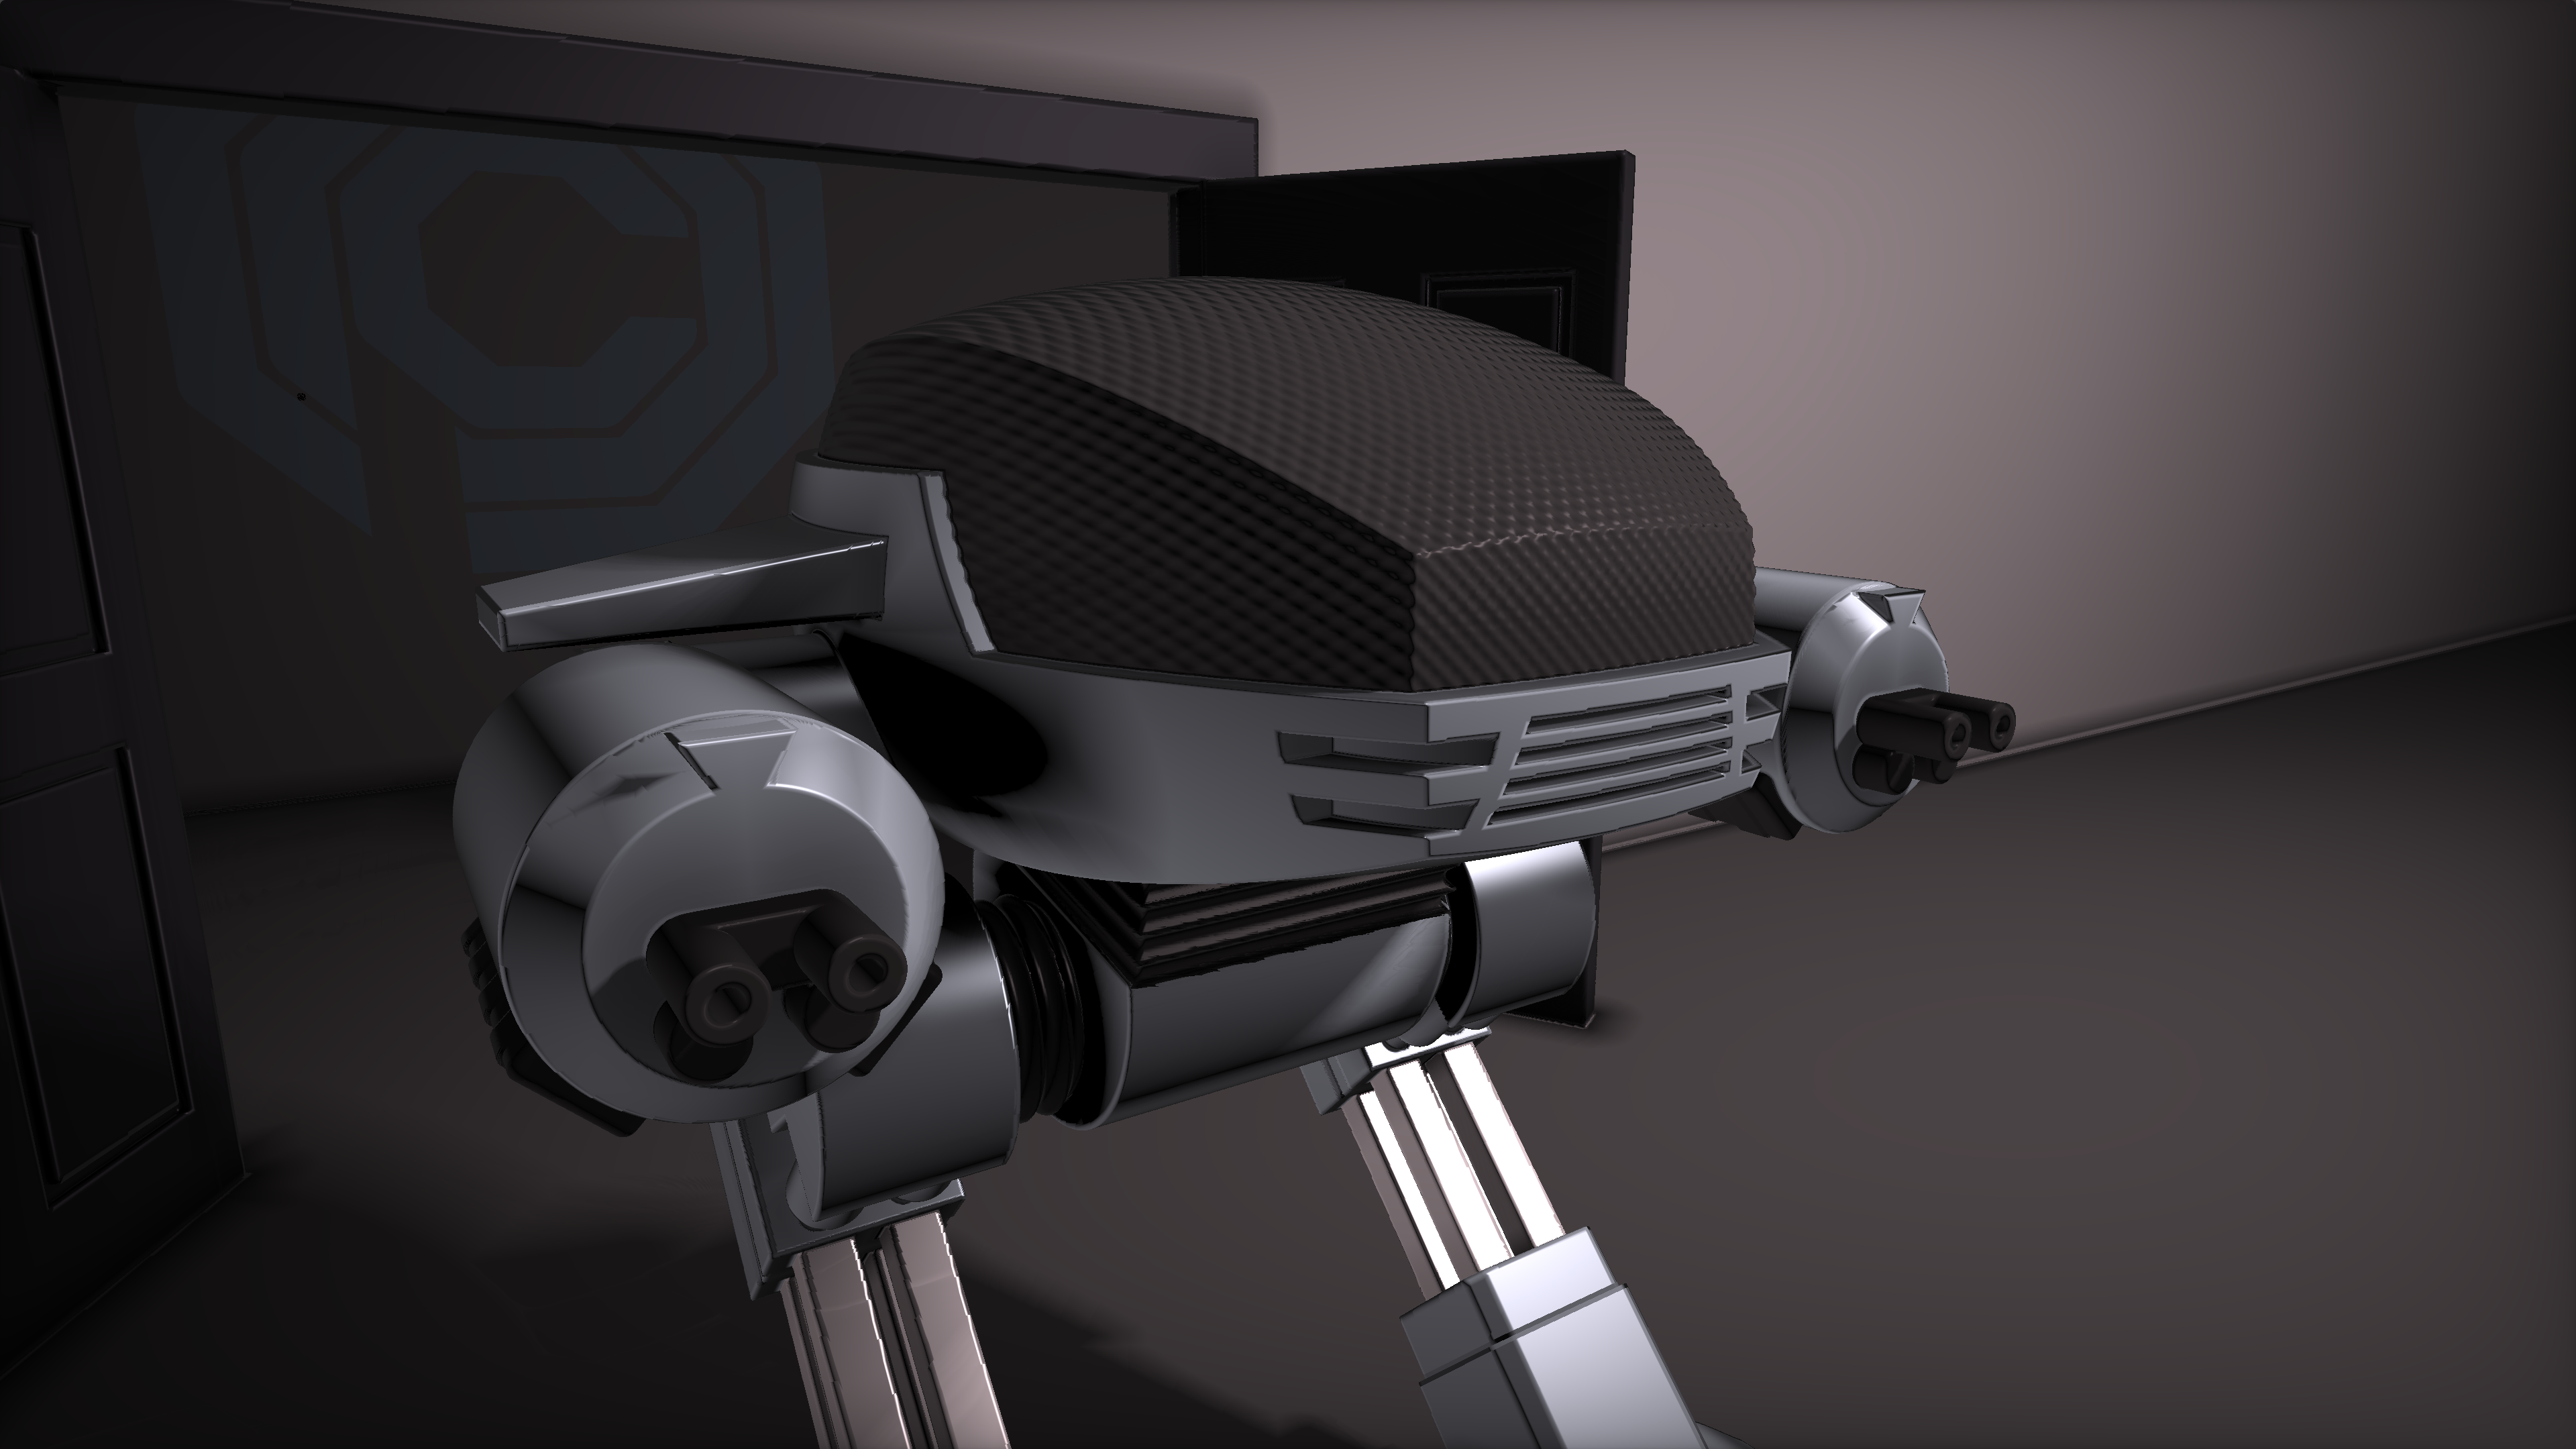
\includegraphics[width=\textwidth]{img/3D/ED-209}
   \caption{\href{https://www.shadertoy.com/view/wsGczG}{ED-209}}
 \end{subfigure}
~
 \begin{subfigure}[b]{0.42\textwidth}
   \includegraphics[width=\textwidth]{img/3D/SpaceAtHome}
   \caption{\href{https://www.shadertoy.com/view/MXS3zy}{Space At Home}}
 \end{subfigure}
 \caption{Propiedad de los respectivos autores}
\end{figure}
\end{columns}
\end{frame}

\begin{frame}{Graficación por computadora en la UNAM}
\begin{columns}
\column[t]{0.5\textwidth}
\begin{itemize}
    \item Ciencias de la Computación
    \begin{itemize}
        \item Animación por Computadora.
        \item Graficación por Computadora
        \item Diseño y Programación de Videojuegos
        \item Realidad Virtual
        \item Visualización
    \end{itemize}
    \item Informática
    \begin{itemize}
        \item Desarrollo de Simulación y Videojuegos
    \end{itemize}
    \item Ingeniería en Computación
    \begin{itemize}
        \item Computación Gráfica e Interacción Humano Computadora
        \item Computación Gráfica Avanzada
    \end{itemize}
\end{itemize}
\column[t]{0.5\textwidth}    
\begin{itemize}
    \item Matemáticas Aplicadas y Computación
    \begin{itemize}
        \item Graficación por Computadora
    \end{itemize}
    \item Tecnologías para la Información en Ciencias
    \begin{itemize}
        \item Visualización 3D de Información Geoespacial
    \end{itemize}
    \item Diseño Gráfico
    \begin{itemize}
        \item Modelado y animación 3D
    \end{itemize}
    \item Diseño y Comunicación Visual
    \begin{itemize}
        \item Arte y Producción para Videojuegos
    \end{itemize}
\end{itemize}
\end{columns}
\end{frame}

\begin{frame}{Creative coding}
\begin{itemize}
    \item Leer \href{https://www.amazon.com/Mathematics-Programming-Computer-Graphics-Third/dp/1435458869}{Mathematics for 3D Game Programming and Computer Graphics} y \href{https://link.springer.com/book/10.1007/978-1-84628-997-2}{Geometric Algebra for Computer Graphics}
    \item Aprender \href{https://en.wikipedia.org/wiki/Computational_geometry}{geometría computacional}.
    \item Aprender un lenguaje de shaders \href{https://www.amazon.com/OpenGL-Shading-Language-Cookbook-high-quality/dp/1789342252/}{como GLSL} a mas profundidad.
    \item Si buscan inspiración a mi me gusta ver el video de \href{https://www.youtube.com/watch?v=BFld4EBO2RE}{Painting a Landscape with Mathematics}
\end{itemize}
\begin{figure}[htp]
 \centering
 \begin{subfigure}[b]{0.3\textwidth}
   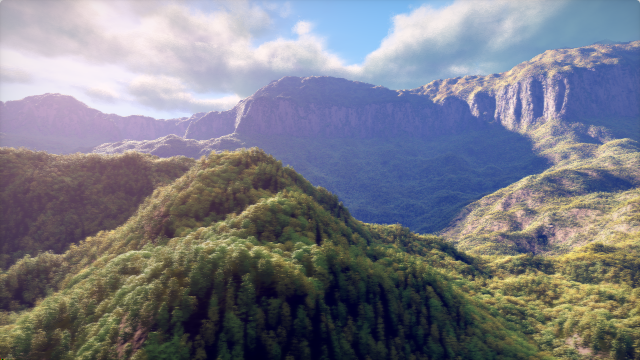
\includegraphics[width=\textwidth]{img/RainForest}
 \end{subfigure}
~
 \begin{subfigure}[b]{0.12\textwidth}
   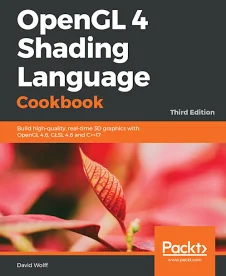
\includegraphics[width=\textwidth]{img/shaderBook}
 \end{subfigure}
\end{figure}
\end{frame}
